
\begin{enumerate}[label=\thesection.\arabic*.,ref=\thesection.\theenumi]
\numberwithin{equation}{enumi}

\item
Given the unity feedback system of Fig. \ref{fig:ee18btech11026_block_1} , with 
\begin{align}
    G(s) = \frac{K}{s(s+5)(s+20)}
\end{align}
The uncompensated system has about 55\% peak overshoot and a peak time if 0.5 seconds when $K_{v} = 10$. Use frequency response technique to design a lead compensator to reduce the percent overshoot to 10\% , while keeping the peak time and steady state error about the same or less.
Consider second order approximations.
\begin{figure}[!ht]
\begin{center}
	\resizebox{\columnwidth}{!}{.\input{./figs/ee18btech11026/ee18btech11026_block_1.tex}}
\end{center}
    \caption{}
    \label{fig:ee18btech11026_block_1}
\end{figure}

\item
\solution

\begin{align}
    K_{v} = \lim_{s \to 0} s G(s) = 10\\
    \implies K = 1000
\end{align}
The bode plot for G(s)is as follows : 

\begin{align}
    G(s) = \frac{1000}{s(s+5)(s+20)}
\end{align}

\begin{figure}[!h]
    \centering
    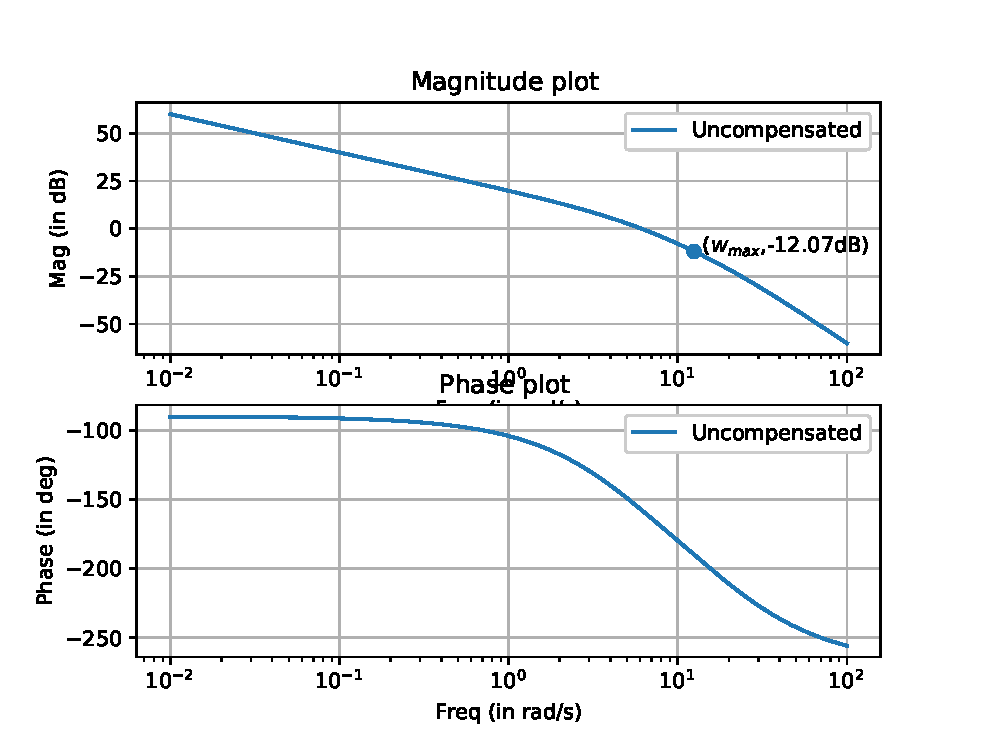
\includegraphics[width=\columnwidth]{./figs/ee18btech11026/ee18btech11026_1.eps}
    \caption{G(s) Bode Plot}
    \label{fig:ee18btech11026_1}
\end{figure}

\begin{align}
    \zeta = \frac{-\ln\left(\frac{OS\%}{100}\right)}{\sqrt{\pi^2+\left(\ln\left(\frac{OS\%}{100}\right)\right)^2}}
\end{align}
\begin{align}
    Phase Margin = \phi_{M} = \tan^{-1}\left(\frac{2\zeta}{\sqrt{-2\zeta^2 + \sqrt{4\zeta^4 + 1}}}\right)  
\end{align}

The following code computes the above quantities.
\begin{lstlisting}
codes/ee18btech11026/ee18btech11026_1.py
\end{lstlisting}


\begin{table}[!ht]
\centering
\input{./tables/ee18btech11026/ee18btech11026_table_1.tex}
\caption{Table of Specifications}
\label{table:ee18btech11026_table_1}
\end{table}
The required additional phase contribution by the compensator will be:
\begin{align}
     \phi_{max} & = 58.9 - 21.16 + correction factor
\end{align}
\begin{align}
     Correction Factor = 25^{\circ}
\end{align}
\begin{align}
    \phi_{max} = 62^{\circ}
\end{align}

\textbf{Note} : Since we know that the lead network will also increase the phase-margin frequency, we add a correction factor to compensate for the lower uncompensated system’s phase angle.Choosing the correction factor is a trail and error procedure so as to reach our expected specifications.\\
The gain compensator's T.F will be of the form:
\begin{align}
    G_{c}(s) = \frac{1}{\beta}\left(\frac{s+\frac{1}{T}}{s+\frac{1}{T\beta}}\right)
\end{align}
This form of T.F does not influence the steady state error.

\textbf{Important Relations to find T and $\beta$}:

\begin{align}
   \phi_{max} = \tan^{-1}\frac{1-\beta}{2\sqrt{\beta}}
\end{align}
The Compensator's magnitude at the phase margin frequency $\omega_{max}$
\begin{align}
     |G_{c}(j\omega_{max})| = \frac{1}{\sqrt{\beta}} 
\end{align}

\begin{align}
    T = \frac{1}{\omega_{max}\sqrt{\beta}}
\end{align}

Using the above formulae :
\begin{align}
    \beta = 0.062\\
    |G_{c}(j\omega_{max})| = 12.07 dB
\end{align}
If we select $\omega_{max}$ to be the new phase-margin frequency, the uncompensated system’s magnitude at this frequency must be -12.07 dB to yield a  0 dB crossover at $\omega_{max}$ for the compensated system.\\
From the bode plot of the un-compensated system, find $\omega_{max}$ where the magnitude is -12.07 dB. This becomes our new phase-margin frequency.
\begin{align}
\omega_{max} = 12.5 rad/sec
\end{align}
\begin{align}
T = 0.321
\end{align}
The Compensator's T.F is as follows :
\begin{align}
G_{c}(s) = 16.13\left(\frac{s + 3.115}{s + 50.25}\right)
\end{align}

The open loop T.F for the compensated system is  :
\begin{align}
    G(s).G_{c}(s) = 16130\left(\frac{(s+3.115)}{s(s+50.25)(s+5)(s+20)}\right)
\end{align}
\item
\textbf{Verification : }
We could observe the  affect of the lead-phase compensator from the phase plots.\\
\begin{figure}[!h]
    \centering
    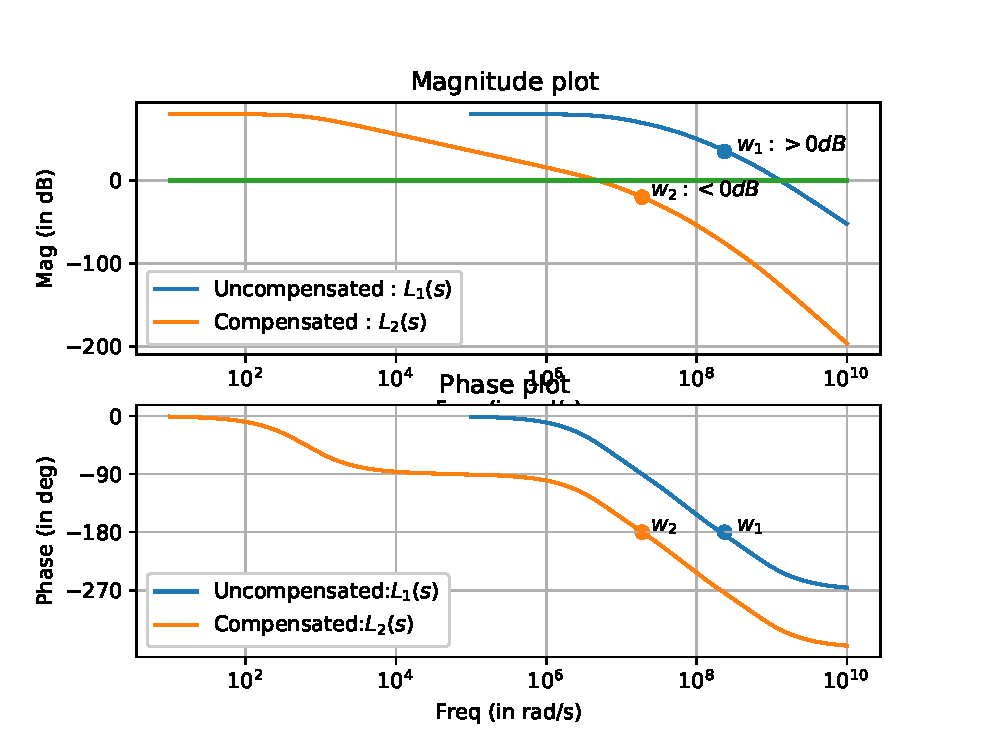
\includegraphics[width=\columnwidth]{./figs/ee18btech11026/ee18btech11026_2.eps}
    \caption{Combined Bode Plots}
    \label{fig:ee18btech11026_2}
\end{figure}


The time responses for a unit step input in a unity feedback system with and without a compensator are as follows : \\
\begin{figure}[!h]
    \centering
    \includegraphics[width=\columnwidth]{./figs/ee18btech11026/ee18btech11026_time.eps}
    \caption{Time response for a unit step input}
    \label{fig:ee18btech11026_time}
\end{figure}



These plots are generated using the below code:
\begin{lstlisting}
codes/ee18btech11026/ee18btech11026_2.py
\end{lstlisting}
\item
\textbf{Result :}
The below is the summary for the designed lead-compensator
\begin{table}[!ht]
\centering
\input{./tables/ee18btech11026/ee18btech11026_table_2.tex}
\caption{Comparing the desired and obtained results}
\label{table:ee18btech11026_table_2}
\end{table}






\end{enumerate}


